\section{Постановка задачи}

\begin{figure}[h!]\centering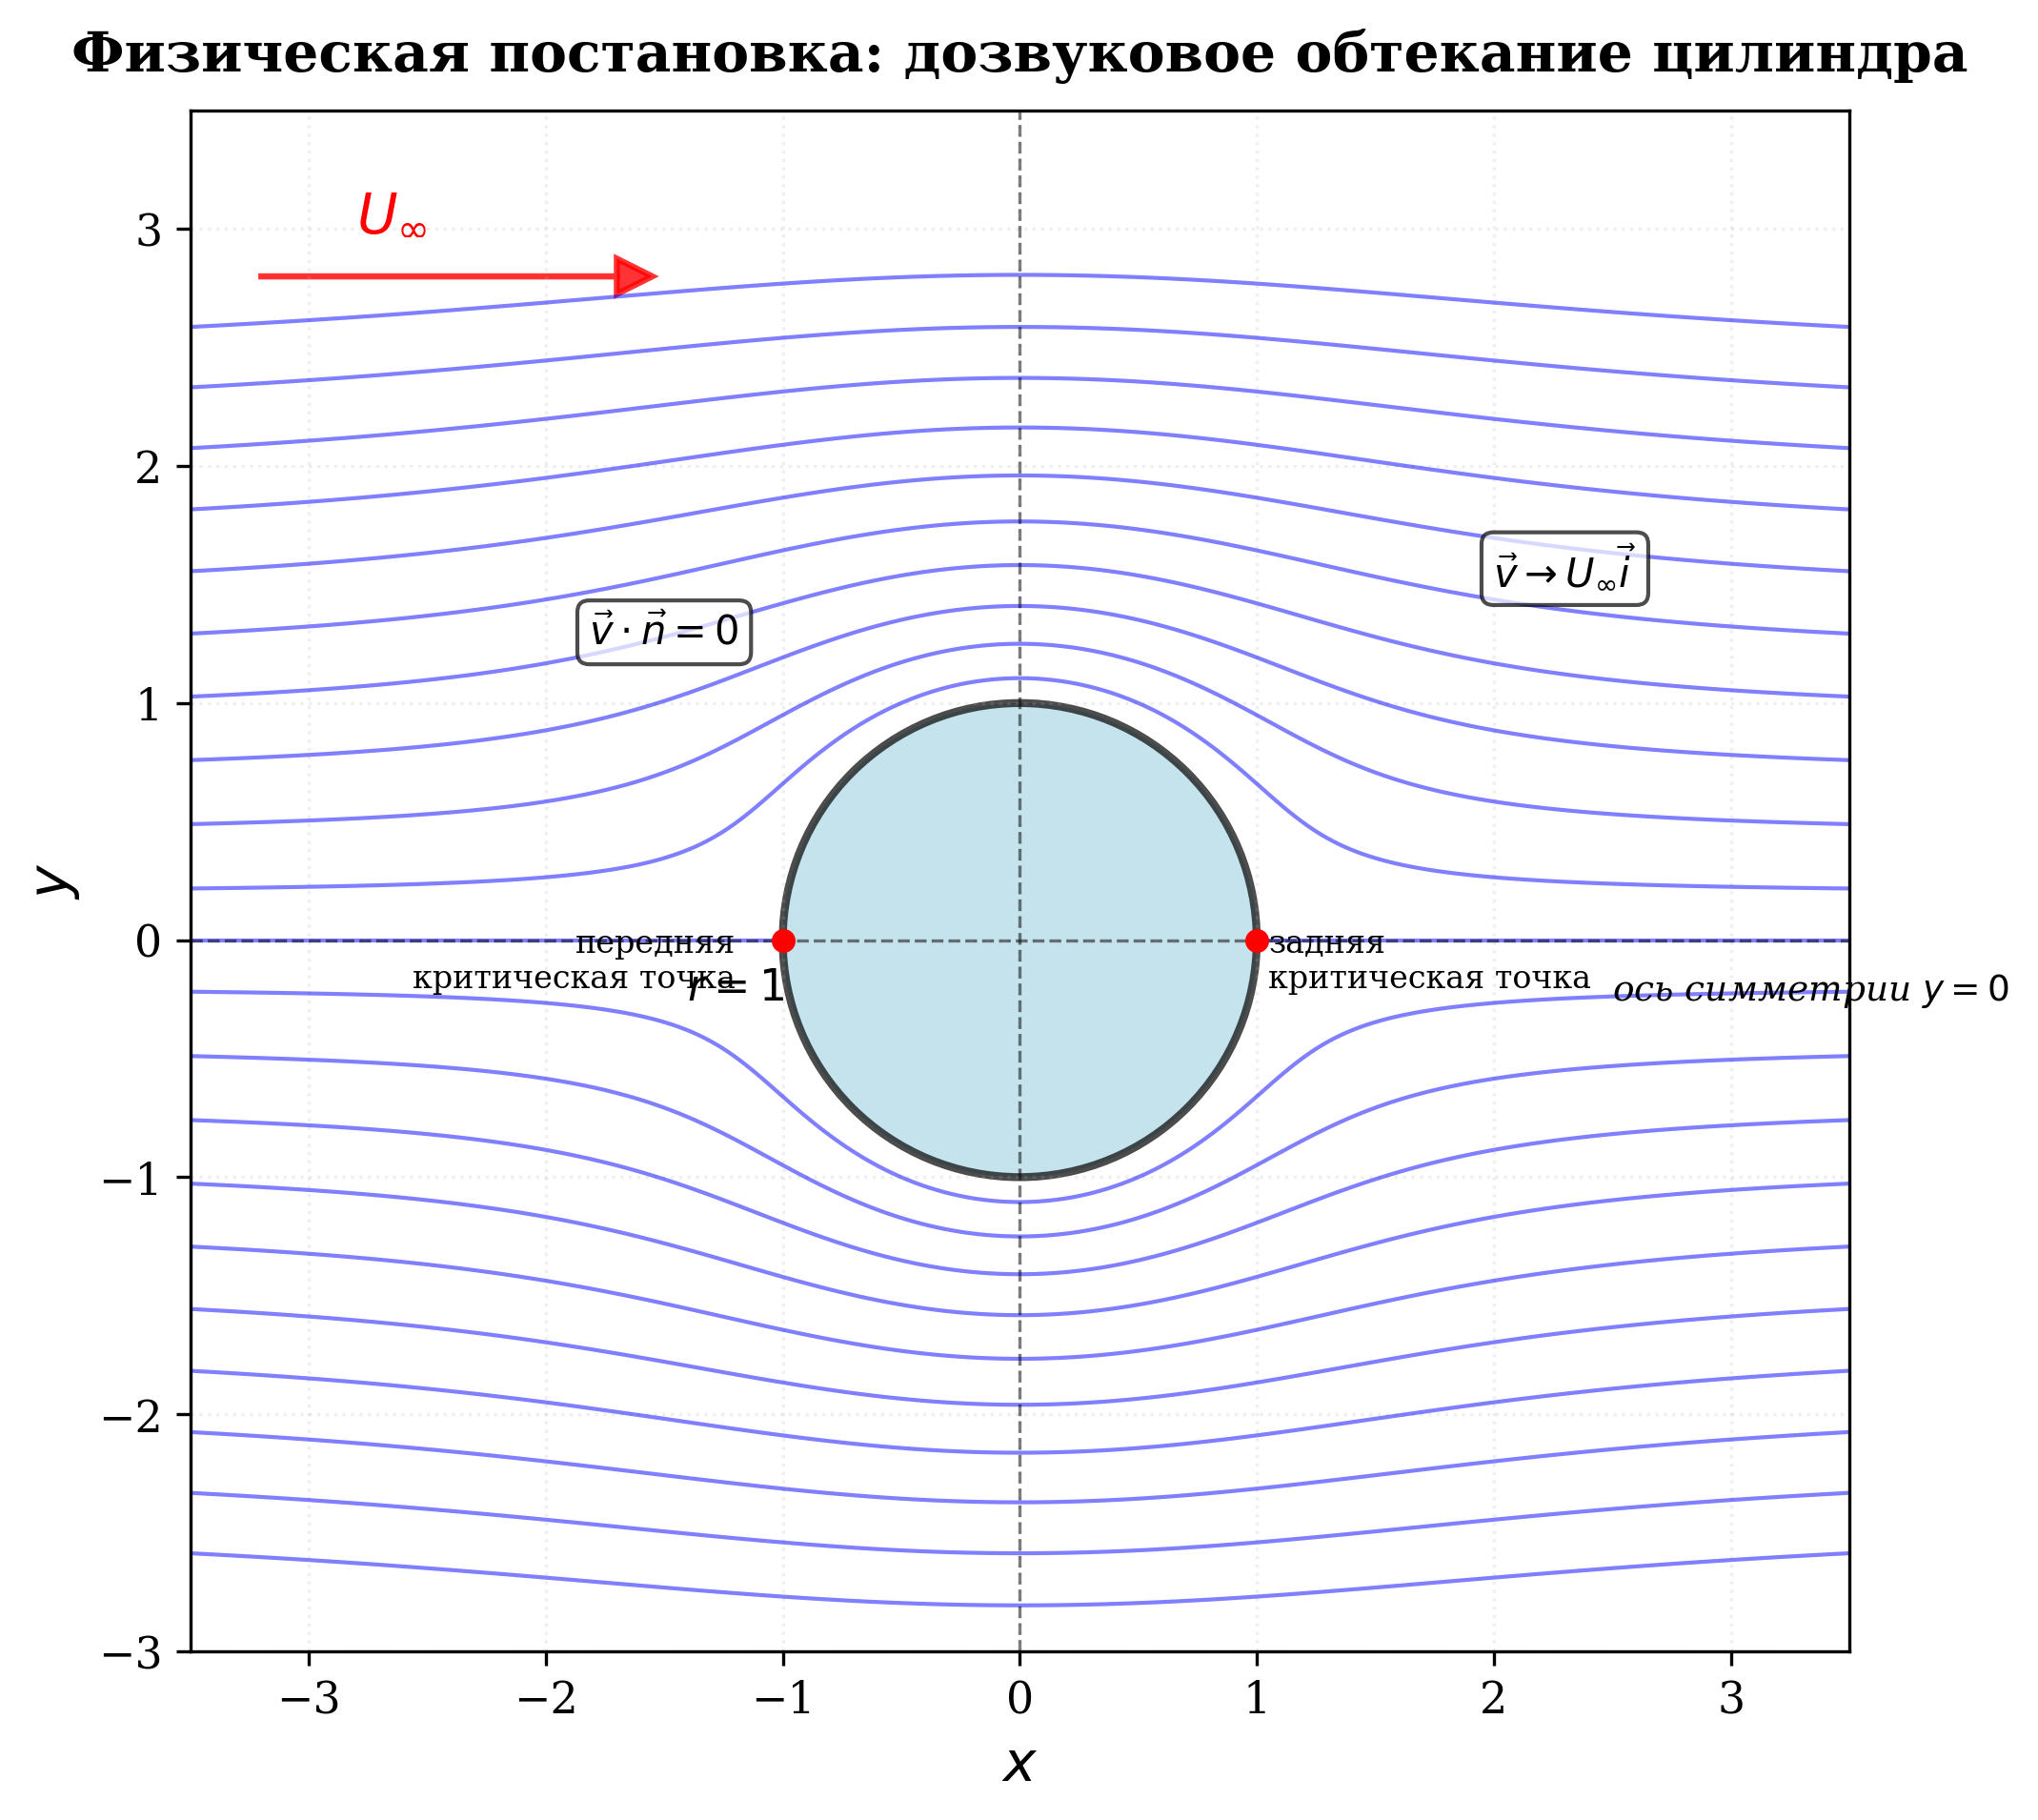
\includegraphics[width=0.4\textwidth]{1_physical_setup.png}\caption{Физическая постановка}\label{fig:setup}\end{figure}
	
	Рассматривается дозвуковое обтекание круглого цилиндра (рис. \ref{fig:setup}). В случае отсутствия завихренности стационарные двумерные уравнения Эйлера можно свести к нелинейному дифференциальному уравнению второго порядка в частных производных относительно потенциала скорости
	
	\[\vec{v} = \nabla \varphi.\]
	В декартовой системе координат имеем уравнение:
	
	\[
		\frac{\partial}{\partial x} \left( \rho \frac{\partial \varphi}{\partial x} \right) + \frac{\partial}{\partial y} \left( \rho \frac{\partial \varphi}{\partial y} \right) = 0,
	\]
	
	где плотность $\rho$ можно получить из условия изэнтропичности.
	
	На оси симметрии, на поверхности цилиндра задается условие непротекания
	
	
	

	\[\vec{v} \cdot \vec{n} = 0. \]	

	
	На больших расстояниях от цилиндра задается условие для невозмущенного потока
	
	
	\[ \vec{v}(r) \to U_{\infty} \vec{i} \quad \text{при} \quad r \to \infty.\]	
	
	
	В рамках данной постановки необходимо исследовать дозвуковое обтекание круглого цилиндра, используя конформное преобразование $\zeta = \ln z$, переводящее внешность единичной окружности на полуполосу $\xi \in [0, +\infty)$, $\eta \in [0, 2\pi]$.
	
	\textbf{Требуется}
	
	В рамках данной работы необходимо выполнить следующие задачи:
	
	\begin{enumerate}
		\item Вывести уравнения и соответствующие граничные условия в системе координат \((\xi, \eta)\).
		\item Составить разностную схему и решить ее с помощью ПНМ (Полностью Неявный Метод),
		сравнить данные по сходимости метода ПНМ с методом релаксации (неявную схема второго
		порядка по поперечной координате).
		\item В расчетной области для различных чисел Маха набегающего потока провести расчеты и сравнить распределение скорости и локального числа Маха.
		\item Исследовать зависимость результатов расчета от параметров сетки.
	\end{enumerate}
	
	\begin{thebibliography}{99}
		\bibitem{bai1961} Бай Ши-и, \textit{Введение в теорию течения сжимаемой жидкости}, ИЛ., М., 1961.
		\bibitem{buleev1959} Булеев Н.И. Численный метод решения двумерных уравнений диффузии // Атомная энергия, 1959, Том 6, № 3, С. 338–340.
		\bibitem{stone1968} Stone H.L. Iterative Solution of Implicit Approximations of Multidimensional Partial Differential Equations // SIAM Journal on Numerical Analysis, 1968, Vol. 5, No. 3, P. 530–558.
		\bibitem{pepper1977} D.W. Pepper, S.D. Harris, Fully Implicit Algorithms for Solving Partial Differential Equations // Journal of Fluids Engineering, 1977, 12, 781–783.
		\bibitem{beloglazkin1992} Белоглазкин А.Н., Шкадов В.Я. О влиянии проницаемости профиля на положение и интенсивность скачка при трансзвуковых скоростях // Вест. Моск. ун-та, сер. 1, математика, механика, 1992, № 5, С. 64–69.
	\end{thebibliography}
	\newpage
